\section{Motivating Examples}

We use \BPGs{} for screening and mitigation of
sepsis in pediatric \textit{Emergency Departments (EDs)}, and management of cardiac arrest
at pediatric Intensive Care Units (ICUs) to illustrate challenges in specifying
BPGs, and developing CGSs for them.

\paragraph{Screening and Mitigation of Sepsis:}

Sepsis is a life threatening condition characterized by an
overwhelming immune response to an injury or infection. In severe cases,
sepsis may lead to organ failure and death. It is
a major cause of morbidity and mortality in children \cite{Eisenberg2021JP}.
Adverse outcomes, however, can be mitigated through early
identification and prompt treatment with antibiotics and
intravenous (IV) fluids \cite{Weiss2014CCM}\cite{Evans2018JAMA}. Thus, early
identification and prompt treatment is vital for managing sepsis. To this end,
guidance systems for automated screening can be employed to detect the onset of
sepsis. Evidence suggests such systems outperform
manual screening \cite{EisenbergAAP21},
leading to their adoption in many \EDs{} \cite{Balamuth2017EM} \cite{Sepanski2014FP}.
Next, we present a \BPG{} for sepsis screening, and use it to identify characteristics
common to \BPGs{} in general.

In \figurename \ref{fig:sepsis-screening}, we present a simplified version of the \BPG{} for
sepsis screening. The \BPG{} specifies the sequence of steps that the \emph{Healthcare
Provider (HCP)} must take in order to evaluate a patient arriving at the \ED{} for
the possibility of sepsis. In essence, when a patient exhibits
a fever or infection, the \HCP{} is supposed to obtain
\begin{enumerate*}[label=(\alph*)]
  \item the patient's age,
  \item any conditions, such as cancer, immunosuppresssion, etc,
    that increase likelihood of sepsis, and
  \item the patient's vital signs, such as heart rate, systolic blood
    pressure, respiratory rate, etc.
\end{enumerate*}


\begin{wraptable}{r}{0.51\textwidth}
  \footnotesize
  \begin{tabular}{ | c || c | c | c | }
    \hline
    \textbf{Age}            & \textbf{Heart Rate}   & \textbf{Systolic BP} & \textbf{Temp}  \\
    \hline
    $0d - 1m$               & $>205$                & $<60$                & $<36 \text{ or } >38$ \\
    \hline
    $\geq 1m - 3m$          & $>205$                & $<70$                & $<36 \text{ or } >38$ \\
    \hline
    $\geq 3m - 1y$          & $>190$                & $<70$                & $<36 \text{ or } >38.5$ \\
    \hline
    $\dots$                 & $\dots$               & $\dots$              & $\dots$ \\
    \hline
    $\geq 13y$              & $>100$                & $<90$                & $<36 \text{ or } >38.5$ \\
    \hline
  \end{tabular}
  \caption{Vital Signs Chart}\label{table:vital-signs}
\end{wraptable}

This information is then used to check for an abnormality
in clusters of linked information, called buckets. For instance, if
the patient's heart rate is abnormal, then bucket 1 is said to
have an abnormal value.
Checking for an abnormality involves use of charts,
such as \tablename{} \ref{table:vital-signs} containing normal ranges indexed by age.
\footnote{For brevity, we omit some age ranges and vital signs from \tablename{} \ref{table:vital-signs}}
If the patient has at least one abnormal value in each of the three buckets,
then he/she is flagged as potentially septic.

\begin{figure}[h]
  \centering
    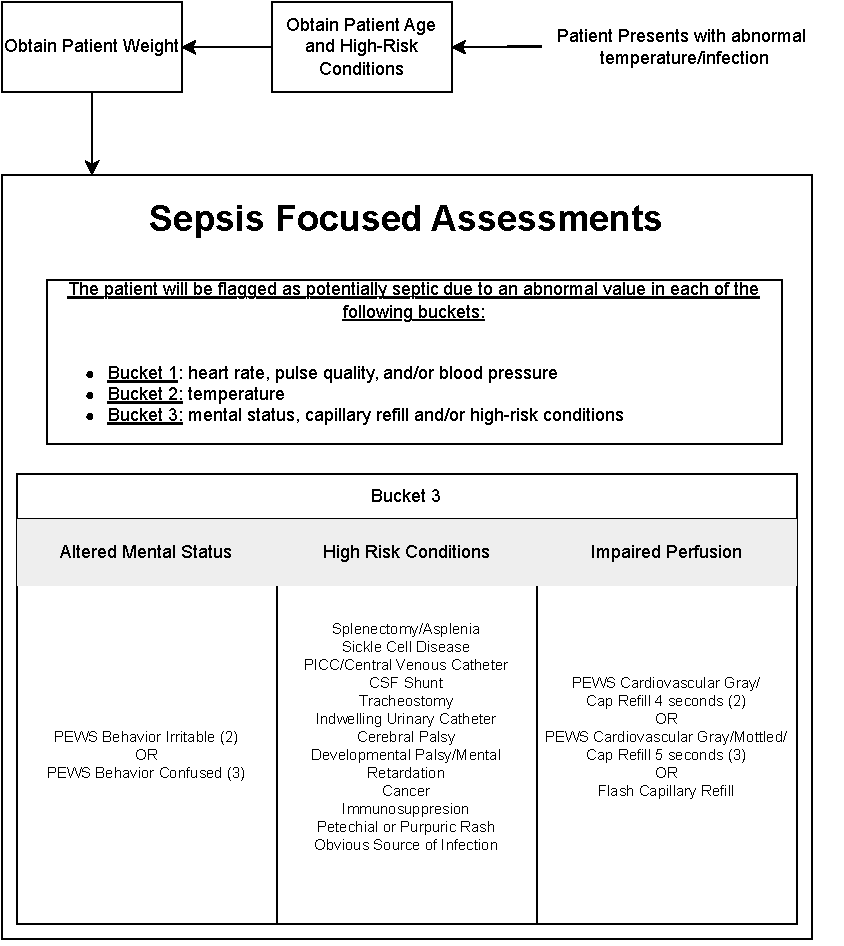
\includegraphics[width=0.75\textwidth]{sepsis-screening-osf}
    \caption{Pediatric Sepsis Screening}\label{fig:sepsis-screening}
\end{figure}

If a patient is flagged as potentially septic, then the guidelines for
sepsis resuscitation should be followed.
It involves multiple \emph{concurrent} workflows, such as
performing diagnostic tests and administering antibiotics.
Fluid Bolus Therapy \emph{(FBT)}, is one such workflow
recommended for sepsis resuscitation \cite{Carcillo2002CCM}. In \figurename
\ref{fig:fluid-therapy}, we provide a version of the \emph{FBT} guidelines used at a
major pediatric hospital. Briefly, if the patient is flagged as
potentially septic, \BPG{} for \emph{FBT} suggests
\begin{enumerate*}[label=(\alph*)]
  \item obtaining any fluid-overdose related risks,
  \item administering normal saline, where the dosage is dictated
    by risks determined in previous step,
  \item waiting for 15 minutes before asking a physician to
    evaluate patient responsiveness.
\end{enumerate*}

If the physician determines that the patient is responding to
administered fluids, then \emph{FBT} can be ended by
shifting the patient to maintainance fluids.
If the patient does not respond to administered fluids and
total fluid administered $\geq 40\ ml/kg$, then ionotropic therapy
should be considered instead. Otherwise, another cycle of
Fluid Bolus Therapy should be followed.

\begin{wrapfigure}[16]{r}{0.5\textwidth}
  \centering
  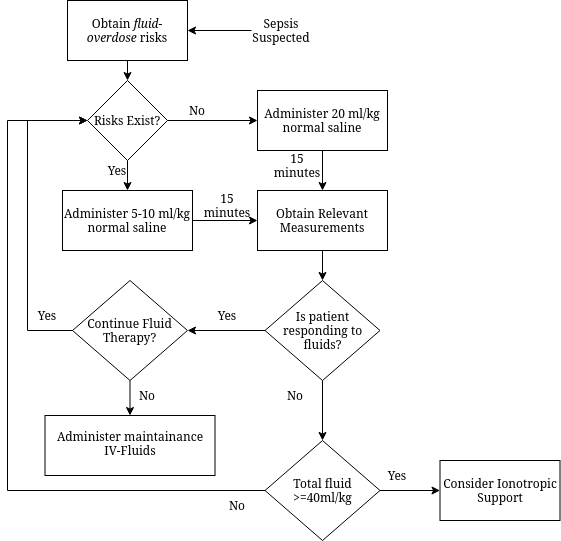
\includegraphics[width=\linewidth]{fluid-therapy}
  \caption{Fluid Bolus Therapy \BPG{}}\label{fig:fluid-therapy}
\end{wrapfigure}

Note the following characteristics exhibited sepsis screening and mitigation \BPG{}:
\begin{itemize}[leftmargin=*]
  \item Comprises \textbf{multiple concurrent} workflows described using
\emph{flowchart}-like notation.
  \item Use \textbf{tables} to depict normal
ranges and values for various parameters such as heart rate, blood pressure etc,
indexed by age or weight.
  \item Relies on \textbf{timing constructs} to instruct the \HCP{} about
    durations of treatments and procedures.
  \item Involves  \textbf{multiple heterogenous agents} such as sensors,
    healthcare records and hospital databases.
\end{itemize}
Next, we describe a \BPG{} for management of cardiac arrest in pediatric \EDs,
and use it to demonstrate that aforementioned characteristics are not
specific to a particular \BPG{}.

\paragraph{Cardiac Arrest Management:}

Cardiac arrest is an abrupt loss of heart function, breath or consciousness.
In-hospital cardiac arrest is common, and associated with high mortality
\cite{AndersenJAMA19}. To mitigate risk of medical errors in managing cardiac
arrest, the American Heart Association (AHA) publishes guidelines that specify
the best practice in managing cardiac arrest, called Advanced Cardiac
Life Support (ACLS). In \figurename \ref{fig:aha-acls},
we show a version of the ACLS \BPG{} from AHA's webiste \cite{acls-url}.
Essentially, the \BPG{} suggests
\begin{enumerate*}[label=(\roman*)]
  \item attaching a defibrilator/monitor and checking if the rhythm is
    shockable,
  \item administering a shock if the rhythm is shockable, followed by
    Cardio Pulmonary Resuscitation (CPR)
    and appropriate medication (like epinephrine), or,
    administering CPR and medication immediately if the rhythm is not shockable.
\end{enumerate*}
The process is repeated based on the rhythm, until spontaneous circulation is restored.

\begin{wrapfigure}{l}{0.5\textwidth}
  \centering
  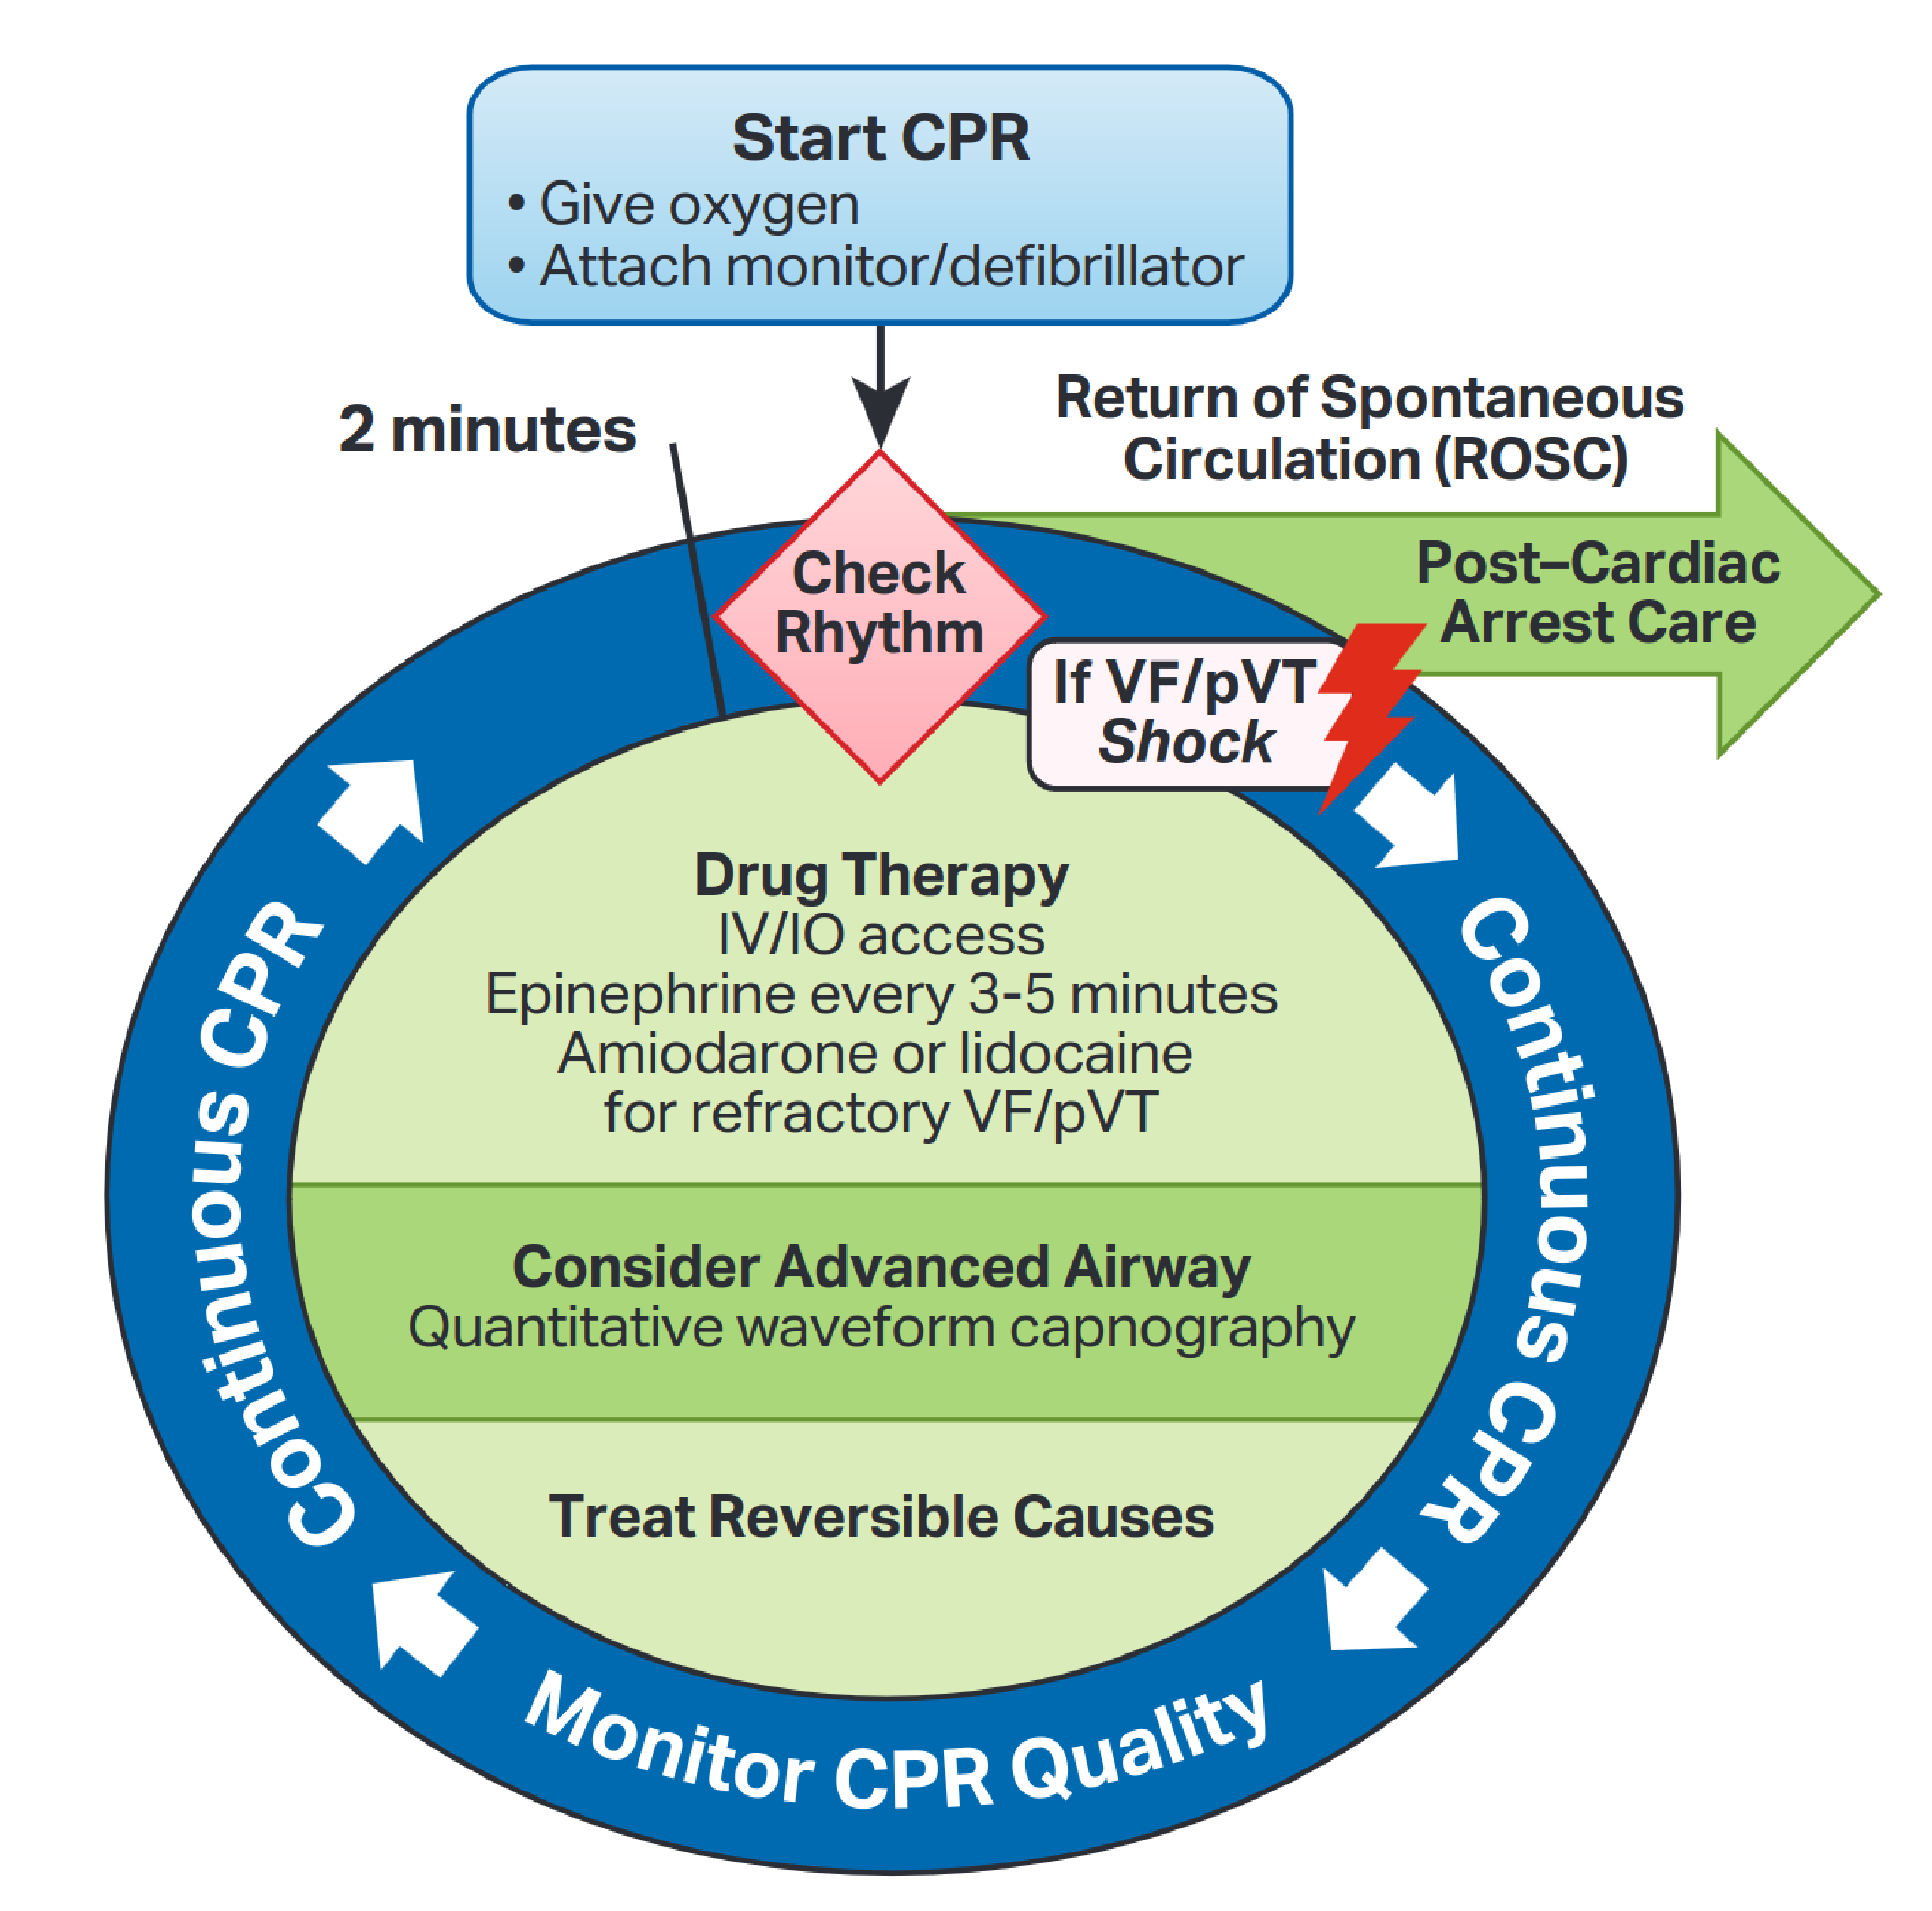
\includegraphics[width=\linewidth]{acls-algorithm}
  \caption{Advanced Cardiac Life Support (ACLS) \BPG{}}\label{fig:aha-acls}
\end{wrapfigure}
